\section{Qué tan confiable es el error}\label{sec:confiabilidad}

Un RMSE de validación cruzada no es todavía el error que tendremos en las 59 parcelas. Revisamos tres cosas.

\textbf{¿La mejora es real o es azar?} La Fig.~\ref{fig:repeticiones} muestra el RMSE de cada una de las 10
repeticiones. El proceso gaussiano gana a la media por régimen y al ridge en 9 de 10. Pero las repeticiones usan las
mismas 138 parcelas, así que no son independientes y contar victorias exagera la evidencia. Con la prueba $t$
corregida de Nadeau y Bengio~\cite{nadeau2003}, la ventaja sobre la media por régimen es de 0.029\,t/ha, con un
intervalo de confianza del 95\,\% de $-0.079$ a $0.022$ ($p=0.26$). La dirección es consistente, pero con 138
parcelas la mejora no alcanza a ser significativa.

\begin{figure}[t]
\centering
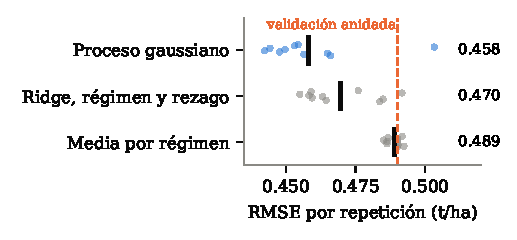
\includegraphics[width=\columnwidth]{f7_repeticiones}
\caption{RMSE de cada repetición del esquema A (puntos) y su promedio (barra). La línea naranja es el error estimado
con validación anidada.}
\label{fig:repeticiones}
\end{figure}

\textbf{¿Cuánto infla el resultado haber elegido el mejor?} Probamos decenas de variantes con las mismas particiones
y nos quedamos con la mejor, lo que favorece a la que tuvo suerte en esas particiones~\cite{cawley2010}. La validación
anidada lo corrige~\cite{varma2006}. En cada fold externo repetimos la elección entre 12 variantes usando solo las
parcelas de entrenamiento, y evaluamos la elegida en el fold externo. El resultado es 0.490\,t/ha, igual que la media
por régimen. La elección interna se repartió entre la media por régimen (6 de 15 folds) y el proceso gaussiano con
rezago a 400\,m (6 de 15). Cambiando la semilla de las particiones, el proceso gaussiano obtiene entre 0.452 y 0.468.
Por eso esperamos un RMSE de 0.46 a 0.49\,t/ha. Las 59 parcelas tienen algo más de vecinos que las de validación
(61\,\% con un vecino a 400\,m o menos, contra 46\,\%), así que el extremo bajo es plausible.

\textbf{¿Hay fuga de información?} Si la etiqueta se filtrara a las variables, el modelo predeciría bien aunque las
etiquetas no tuvieran sentido. Lo probamos revolviendo los rendimientos dentro de cada régimen, lo que conserva el
régimen pero rompe la relación con los vecinos (Fig.~\ref{fig:permutacion}). Con las etiquetas revueltas el modelo
nunca baja de 0.488, y con las reales obtiene 0.467 en las mismas condiciones. Revolviendo entre todas las parcelas, el
modelo queda en 0.861, peor que la media global (0.855). El rezago capta una relación real entre vecinos.

\begin{figure}[t]
\centering
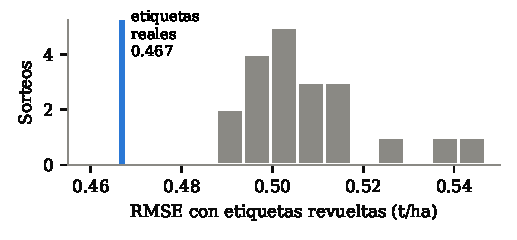
\includegraphics[width=\columnwidth]{f8_permutacion}
\caption{RMSE del modelo en 20 sorteos con los rendimientos revueltos dentro de cada régimen, contra el RMSE con los
rendimientos reales.}
\label{fig:permutacion}
\end{figure}

\textbf{Margen por calificar con 59 parcelas.} Aun con el modelo correcto, el RMSE de 59 parcelas varía según cuáles
toquen. Sorteamos 5000 grupos de 37 errores del régimen A y 22 del B, como en la partición oficial
(Fig.~\ref{fig:margen}). El 90\,\% de los sorteos cae entre 0.35 y 0.56\,t/ha. Este margen es mayor que la diferencia
entre cualquiera de los modelos que comparamos.

\begin{figure}[t]
\centering
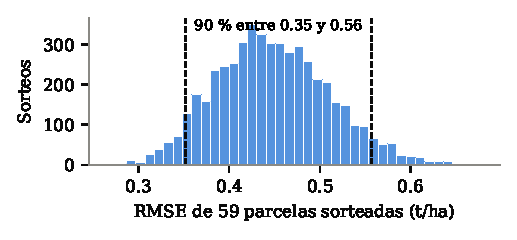
\includegraphics[width=\columnwidth]{f9_margen}
\caption{RMSE de 5000 grupos de 59 parcelas sorteados entre los errores fuera de fold del modelo.}
\label{fig:margen}
\end{figure}
